% Source: Lecture5.pdf, pages 1-6 (pages 7-10 are blank). The file has no
% lecture heading; it follows Lecture 4 in the numbering of the files.
\lecture{5}
\subsection{Thermodynamic energy functions}

Here we review basic energy functions from thermodynamics. We begin with variables for
liquid--gas--solid, then with a magnetic system.

\paragraph{Internal energy $U$.} This increases due to heat $\dd Q = T\dd S$ added to a
system and decreases due to the work $\dd W = p\,\dd V$ by the system. So
$\dd U = T\dd S - p\,\dd V$. One writes $U = U(S,V)$ and identifies the partial derivatives
$(\partial U/\partial S)_V = T$ and $(\partial U/\partial V)_S = -p$, so
\begin{equation}
  \dd U = \left(\pder{U}{S}\right)_V\dd S + \left(\pder{U}{V}\right)_S\dd V
\end{equation}
(subscripts are included here, but not necessary).

\paragraph{Legendre transform.} Given a differentiable function $f(x,y)$ with
\begin{equation}
  \dd f = \left(\pder{f}{x}\right)_y\dd x + \left(\pder{f}{y}\right)_x\dd y \equiv u\,\dd x + v\,\dd y
\end{equation}
(do not confuse $u$ with capital $U$), we can construct a Legendre transform of $f$,
namely $g(u,y)$, as follows: let $g = f - ux$; then
\begin{equation}
  \dd g = \dd f - \dd(ux) = u\,\dd x + v\,\dd y - (u\,\dd x + x\,\dd u)
        = -x\,\dd u + v\,\dd y
        = \left(\pder{g}{u}\right)_y\dd u + \left(\pder{g}{y}\right)_u\dd y,
\end{equation}
with $(\partial g/\partial u)_y = -x$ and $(\partial g/\partial y)_u = v$. This procedure
replaces the variable $x$ by the variable $u$. We will apply this Legendre transform 3
times to construct 3 more useful energy functions.

\paragraph{Enthalpy,} a function of $S$ and $p$. This function is used especially in
chemistry and engineering, where it is denoted $H$. In statistical physics, the symbol $H$
is conventionally reserved for the external magnetic field, so we have to use a different
symbol. Stanley uses $E$; we will use $H_e$, where the subscript ``e'' stands for
``enthalpy''. Let $H_e = U + pV$; then
\begin{equation}
  \dd H_e = \dd U + \dd(pV) = T\dd S - p\,\dd V + p\,\dd V + V\dd p = T\dd S + V\dd p,
\end{equation}
so $H_e = H_e(S,p)$, with $(\partial H_e/\partial S)_p = T$ and
$(\partial H_e/\partial p)_S = V$.

\paragraph{Gibbs free energy $G = G(T,p)$.} Let $G = H_e - TS$, so
\begin{equation}
  \dd G = \dd H_e - \dd(TS) = T\dd S + V\dd p - T\dd S - S\dd T = -S\dd T + V\dd p,
\end{equation}
so $(\partial G/\partial T)_p = -S$ and $(\partial G/\partial p)_T = V$. This energy
function is especially useful, because it depends on the two variables that we control
experimentally, temperature $T$ and pressure $p$.

\paragraph{Helmholtz free energy $A = A(T,V)$.} Let $A = U - TS$;
\begin{equation}
  \dd A = \dd U - \dd(TS) = T\dd S - p\,\dd V - T\dd S - S\dd T = -S\dd T - p\,\dd V,
\end{equation}
so $(\partial A/\partial T)_V = -S$ and $(\partial A/\partial V)_T = -p$.

\paragraph{Magnetic systems.} Now define the corresponding energy functions for a magnetic
system. A difference is that if one exerts an external pressure $p$ on a system, it causes
the volume $V$ of the system to decrease, while if one applies an external magnetic field
to a system, it increases the induced magnetization (in the direction of the applied
field). This difference leads to some opposite minus signs. So the correspondence is:
\begin{itemize}
  \item $p$ in solid--liquid--gas $\leftrightarrow$ $H$ in a magnetic system (with reversal
    of sign);
  \item $V$, the property of the system affected by $p$ $\leftrightarrow$ $M$, the property
    of the system affected by $H$.
\end{itemize}

\subsubsection*{Summary of energy functions}

\begin{center}
\renewcommand{\arraystretch}{1.3}
\begin{tabular}{l|l}
  solid--liquid--gas & magnetic\\ \hline
  $U = U(S,V)$,\quad $\dd U = T\dd S - p\,\dd V$ & $U = U(S,M)$,\quad $\dd U = T\dd S + H\dd M$\\
  $H_e = H_e(S,p)$,\quad $\dd H_e = T\dd S + V\dd p$ & $H_e = H_e(S,H)$,\quad $\dd H_e = T\dd S - M\dd H$\\
  $G = G(T,p)$,\quad $\dd G = -S\dd T + V\dd p$ & $G = G(T,H)$,\quad $\dd G = -S\dd T - M\dd H$\\
  $A = A(T,V)$,\quad $\dd A = -S\dd T - p\,\dd V$ & $A = A(T,M)$,\quad $\dd A = -S\dd T + H\dd M$
\end{tabular}
\end{center}

\subsection{Maxwell relations}

Let $f = f(x,y)$;
$\dd f = (\partial f/\partial x)_y\dd x + (\partial f/\partial y)_x\dd y
\equiv\xi(x,y)\dd x + \eta(x,y)\dd y$. For a nonsingular function,
\begin{equation}
  \pder{\xi}{y} = \pder{}{y}\left(\pder{f}{x}\right) = \frac{\partial^2 f}{\partial y\,\partial x}
  = \frac{\partial^2 f}{\partial x\,\partial y} = \pder{}{x}\left(\pder{f}{y}\right) = \pder{\eta}{x}.
\end{equation}
Apply these relations, first for the solid--liquid--gas system:
\begin{align}
  U:&\quad T = \left(\pder{U}{S}\right)_V,\ -p = \left(\pder{U}{V}\right)_S
     &&\Rightarrow\quad \left(\pder{T}{V}\right)_S = \left(\pder{(-p)}{S}\right)_V = -\left(\pder{p}{S}\right)_V,\\
  H_e:&\quad T = \left(\pder{H_e}{S}\right)_p,\ V = \left(\pder{H_e}{p}\right)_S
     &&\Rightarrow\quad \left(\pder{T}{p}\right)_S = \left(\pder{V}{S}\right)_p,\\
  G:&\quad -S = \left(\pder{G}{T}\right)_p,\ V = \left(\pder{G}{p}\right)_T
     &&\Rightarrow\quad -\left(\pder{S}{p}\right)_T = \left(\pder{V}{T}\right)_p,\\
  A:&\quad -S = \left(\pder{A}{T}\right)_V,\ -p = \left(\pder{A}{V}\right)_T
     &&\Rightarrow\quad \left(\pder{S}{V}\right)_T = \left(\pder{p}{T}\right)_V.
\end{align}
Corresponding Maxwell relations apply for magnetic systems; there is a summary in the
front cover of Stanley's book (hardcover); see the photocopy as the file ``stanleycover''
on Blackboard.

\subsection{Canonical ensemble and partition function}

A very useful object in stat.\ mech.\ is the canonical ensemble and the associated
partition function. Consider a system in thermal equilibrium at temperature $T$. One
observes that the probability $P_r$ that the system is in a state $r$ with energy $E_r$ is
\begin{equation}
  P_r = c\,e^{-\beta E_r},\qquad\text{where}\quad \beta\equiv\frac{1}{\kB T},
\end{equation}
and the constant $c$ is determined by the fact that the sum of the $P_r$ over all $r$ is 1:
$\sum_r P_r = 1 = c\sum_r e^{-\beta E_r}$, so $c = 1/\sum_r e^{-\beta E_r}$, and hence
\begin{equation}
  P_r = \frac{e^{-\beta E_r}}{\sum_r e^{-\beta E_r}}.
\end{equation}
N.B.: if the states form a continuum, the sum is replaced by an integral. Physically, if
$T\to\infty$ ($\beta\to 0$), all states are equally probable; if $T\to 0$, the state(s)
with lowest energy are preferentially occupied.

It is thus convenient to define the function
\begin{equation}
  Z = \sum_r e^{-\beta E_r},
\end{equation}
which contains much information about the system. This is called the partition function;
the symbol $Z$ comes from German, for ``Zustandssumme'' (``state-sum''). The average
internal energy $U$ is
\begin{equation}
  U = \sum_r E_rP_r = \frac{\sum_r E_r e^{-\beta E_r}}{\sum_r e^{-\beta E_r}}
    = -\pder{}{\beta}\ln Z = -\frac{\partial Z/\partial\beta}{Z}.
\end{equation}
The energy in a given state $r$ is determined by the Hamiltonian $\Ham$ (script $\Ham$ to
avoid confusion with the magnetic field $H$), so one can write simply
\begin{equation}
  Z = \sum_{\text{states}}e^{-\beta\Ham}.
\end{equation}
This is the canonical ensemble.

\subsection{The thermodynamic limit}

In stat.\ mech.\ one defines a formal limit, the ``thermodynamic limit'', by letting the
volume $V\to\infty$, the number of sites on a lattice $\to\infty$, or the number of
atoms/molecules in a gas, liquid, or solid $\to\infty$ with a fixed number density $N/V$.
In this limit, one naturally deals with the energy per unit volume or per site or particle,
\begin{equation}
  \bar U = \lim_{\text{therm.}}\frac{U}{N},
\end{equation}
since this is finite in the thermodynamic limit. Hence, we define a reduced dimensionless
free energy function
\begin{equation}
  f = \lim_{N\to\infty}\frac1N\ln Z,\qquad\text{so}\quad \bar U = -\pder{f}{\beta}.
\end{equation}
The corresponding Gibbs free energy per volume or per particle is $\bar G = -\kB Tf$. We
will often drop the bar on $\bar U$, $\bar G$ and other quantities such as $\bar M$ when
the context makes clear that we are considering these quantities in the thermodynamic limit
(intensive; extensive).

Boundary conditions (BC): in $d = 1$, free (FBC) or periodic (PBC), where the chain
closes on itself in a ring; in $d = 2$, free, cylindrical or toroidal.

For a magnetic system, say the Ising system with $\sigma_i = \pm 1$ (\# states $= 2^N$),
\begin{equation}
  \Ham = -J\sum_{\langle ij\rangle}\sigma_i\sigma_j - H\sum_i\sigma_i,\qquad
  Z = \sum_{\{\sigma_i\}}e^{-\beta\Ham}
    = \sum_{\{\sigma_i\}}e^{K\sum_{\langle ij\rangle}\sigma_i\sigma_j + h\sum_i\sigma_i},
\end{equation}
where $K\equiv\beta J$ and $h\equiv\beta H$, so
\begin{equation}
  \bar M = \ev{\sigma_i} = \frac1\beta\pder{f}{H} = \pder{f}{h}.
\end{equation}
The spontaneous magnetization is
\begin{equation}
  \bar M_{sp} = \lim_{H\to 0}\pder{f}{h}.
\end{equation}

\subsection{The one-dimensional Ising model}

We illustrate these concepts with a simple system, the 1D Ising model. N.B.: this system
(1) does not exhibit a phase transition at finite temperature; (2) $\exists$ a phase
transition at $T = 0$; (3) the non-analyticities in thermodynamic functions are not of
algebraic form; (4) the phase transition has both continuous and discontinuous
singularities.
\begin{equation}
  \Ham = -J\sum_{\langle ij\rangle}\sigma_i\sigma_j - H\sum_i\sigma_i,\qquad
  -\beta\Ham = K\sum_{\langle ij\rangle}\sigma_i\sigma_j + h\sum_i\sigma_i,\qquad
  Z = \sum_{\{\sigma_i\}}e^{-\beta\Ham}
\end{equation}
with $2^N$ states. To compute $Z$, we will use a transfer matrix method. The matrix element
of the transfer matrix $T$ (not temperature) is
\begin{equation}
  \langle\sigma_{i+1}|T|\sigma_i\rangle = e^{K\sigma_{i+1}\sigma_i + \frac{h}{2}(\sigma_{i+1}+\sigma_i)}.
\end{equation}
For the spin states $++$, $-+$, $+-$, $--$:
\begin{equation}
  \langle +|T|+\rangle = e^{K+h},\quad
  \langle -|T|+\rangle = e^{-K},\quad
  \langle +|T|-\rangle = e^{-K},\quad
  \langle -|T|-\rangle = e^{K-h},
\end{equation}
so
\begin{equation}
  T = \begin{pmatrix} e^{K+h} & e^{-K}\\ e^{-K} & e^{K-h}\end{pmatrix}.
\end{equation}
$T$ is a real symmetric matrix $\Rightarrow\exists$ an orthogonal transformation
$\mathcal{O}$: $\mathcal{O}T\mathcal{O}^{-1} = T_d$, $T = \mathcal{O}^{-1}T_d\mathcal{O}$
(recall the definition of an orthogonal matrix: $\mathcal{O}^T = \mathcal{O}^{-1}$). With
PBC, $\sigma_{N+1}\equiv\sigma_1$, the sites forming a ring,
\begin{align}
  Z &= \sum_{\{\sigma_i\}}\langle\sigma_1|T|\sigma_N\rangle\cdots\langle\sigma_2|T|\sigma_1\rangle
     = \sum_{\{\sigma_i\}}\langle\sigma_1|\mathcal{O}^{-1}T_d\mathcal{O}|\sigma_N\rangle\cdots
       \langle\sigma_2|\mathcal{O}^{-1}T_d\mathcal{O}|\sigma_1\rangle\nonumber\\
    &= \Tr(T_d^N),
\end{align}
where we use the property $\Tr(AB) = \Tr(BA)$. So the next step is to diagonalize the
transfer matrix $T$.

\subsubsection*{Diagonalization of the transfer matrix}

First, do this for $H = 0$, i.e.\ no external magnetic field:
\begin{equation}
  T = \begin{pmatrix} e^{K} & e^{-K}\\ e^{-K} & e^{K}\end{pmatrix},\qquad
  (\lambda - e^K)(\lambda - e^K) - e^{-2K} = 0,\qquad
  \lambda^2 - 2e^K\lambda + (e^{2K}-e^{-2K}) = 0,
\end{equation}
\begin{equation}
  \lambda_\pm = \tfrac12\left[2e^K\pm\sqrt{4e^{2K}-4(e^{2K}-e^{-2K})}\right]
  = e^K\pm e^{-K} = \begin{cases} 2\cosh K\\ 2\sinh K.\end{cases}
\end{equation}
We use the notation $\cosh K\equiv\operatorname{ch}K$, $\sinh K\equiv\operatorname{sh}K$,
$\tanh K\equiv\operatorname{th}K$, and
\begin{equation}
  v\equiv\tanh K .
\end{equation}
Then $T_d = \operatorname{diag}(\lambda_+,\lambda_-)$ and
\begin{equation}
  Z = \lambda_+^N + \lambda_-^N = 2^N\left[(\cosh K)^N + (\sinh K)^N\right]
    = 2^N(\cosh K)^N\left[1 + v^N\right],
\end{equation}
\begin{equation}
  \ln Z = N\ln 2 + N\ln[\cosh K] + \ln[1+v^N],
\end{equation}
\begin{equation}
  f = \lim_{N\to\infty}\frac1N\ln Z = \ln 2 + \ln(\cosh K) = \ln[2\cosh K] = \ln(\lambda_{\max});
  \qquad \bar G = -\kB Tf .
\end{equation}
So
\begin{equation}
  \bar U = -\pder{f}{\beta} = -J\pder{f}{K} = -J\tanh K = -Jv = -J\ev{\sigma_1\sigma_2}.
\end{equation}
Note $\tanh(-x) = -\tanh x$; $J\to -J$ means $K\to -K$.

\begin{diagram}
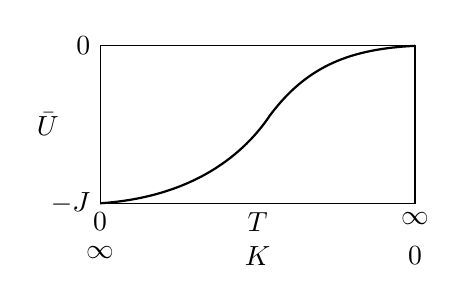
\begin{tikzpicture}[scale=0.8]
  \draw (0,0) rectangle (5,2.5);
  \draw[thick] (0,0) .. controls (1.5,0.1) and (2.3,0.8) .. (2.7,1.4) .. controls (3.3,2.2) and (4,2.45) .. (5,2.5);
  \node[left] at (0,2.5) {$0$}; \node[left] at (0,0) {$-J$};
  \node[left] at (-0.5,1.25) {$\bar U$};
  \node[below] at (0,0) {$0$}; \node[below] at (5,0) {$\infty$}; \node[below] at (2.5,0) {$T$};
  \node[below=12pt] at (0,0) {$\infty$}; \node[below=12pt] at (5,0) {$0$}; \node[below=12pt] at (2.5,0) {$K$};
\end{tikzpicture}
\diagramcaption{Internal energy per site of the 1D Ising ferromagnet.}
\end{diagram}
